\chapter{Workload Breakdown}
In addition to the times, the duration and the task variance are calculated with the following formulas. 
\\
\[duration = \dfrac{pessimistic + 4 * most\, likely + optimistic}{6}\]
\[task\, variance = \dfrac{2 * (pessimistic - optimistic)}{6}\]
\subsection*{Project Managment Report [Prmr]}
\label{sec:orgd96ec13}
\begin{center}
\begin{tabular}{|l|r|}
	\hline
	 & Time in hours\\
	 \hline
	optimistic & 65\\
	\hline
	most likely & 92\\
	\hline
	pessimistic & 130\\
	\hline
	\hline
	duration & 93.3\\
	\hline
	task variance & 21.7\\
	\hline
\end{tabular}
\end{center}
\begin{itemize}
\item create product requirement catalog (50 / 70 / 100)
\item create GANTT diagram (5 /10 / 15)
\item negoitate time and costs with customer (10 / 12 /15 )
\end{itemize}

\subsection*{Hardware prerequisites [Hpre]}
\label{sec:orgfb33f5b}

\begin{center}
	\begin{tabular}{|l|r|}
		\hline
		& Time in hours\\
		\hline
		optimistic & 108\\
		\hline
		most likely & 182\\
		\hline
		pessimistic & 256\\
		\hline
		\hline
		duration & 182\\
		\hline
		task variance & 49.3\\
		\hline
	\end{tabular}
\end{center}


\subsubsection*{Video cameras [HpreCam]}
\label{sec:org3a27049}
	\begin{enumerate}
	\item research for good product
	\begin{itemize}
	\item investigate environment / areas / building (8/10/12)
	\item estimate amounts and total costs (8/10/12)
	\end{itemize}
	\item negotiate with customer (8/10/12)
	\item buy those products (8/10/12)
	\end{enumerate}

\subsubsection*{Storage [HpreS]}
\label{sec:orgeb93f9e}
\begin{enumerate}
\item research archive backup file system
\begin{itemize}
\item NAS with redundance (RAID 2) (4/6/8)
\item Backup also with (RAID 2) (4/6/8)
\end{itemize}
\end{enumerate}

\subsubsection*{Panels [HpreP]}
\label{sec:org4b41c6c}
\begin{enumerate}
\item research for good product
\begin{itemize}
\item investigate environment / areas / building (8/10/12)
\item estimate amounts and total costs (4/8/12)
\end{itemize}
\item negotiate with customer (4/8/12)
\item buy those products (4/8/12)
\end{enumerate}

\subsubsection*{Control Unit (PLC) [HprePLC]}
\label{sec:orgd40ef86}
\begin{enumerate}
\item research for good product
\begin{itemize}
\item investigate environment / areas / building (4/8/12)
\item estimate amounts and total costs (4/8/12)
\end{itemize}
\item negotiate with customer (4/8/12)
\item buy those products (4/8/12)
\end{enumerate}

\subsubsection*{Server [HpreSer]}
\label{sec:org7b31fb6}
\begin{enumerate}
\item research for good product
\begin{itemize}
\item investigate environment / areas / building (4/8/12)
\item estimate amounts and total costs (4/8/12)
\end{itemize}
\item negotiate with customer (4/8/12)
\item buy those products (4/8/12)
\end{enumerate}
\subsubsection*{Sensors [HpreSens]}
\label{sec:org6352bec}

\begin{enumerate}
\item research for good product
\begin{itemize}
\item investigate environment / areas / building (4/8/12)
\item estimate amounts and total costs (4/8/12)
\end{itemize}
\item negotiate with customer (4/8/12)
\item buy those products (4/8/12)
\end{enumerate}



\subsection*{Hardware installation [Hin]}
\label{sec:org2cae8f9}

\begin{center}
\begin{tabular}{|l|r|}
	\hline
	& Time in hours\\
	\hline
	optimistic & 40\\
	\hline
	most likely & 50\\
	\hline
	pessimistic & 60\\
	\hline
	\hline
	duration & 50\\
	\hline
	task variance & 6.7\\
	\hline
\end{tabular}
\end{center}

\subsubsection*{installation and configuration}
\label{sec:org7c12187}
\begin{itemize}
\item video cameras (8/10/12) [HinCam] 
	\begin{itemize}
	\item dependent on [HpreCam]
	\end{itemize}
\item storage  (8/10/12)[HinS]
	\begin{itemize}
	\item dependent on [HpreS, HpreCam]
	\item connect video cameras to system
	\end{itemize}
\item panels (8/10/12)[HinP]
	\begin{itemize}
	\item dependent on [HpreP]
	\item configuration
	\end{itemize}
\item Control Unit (PLC) (8/10/12) [HinPLC]
	\begin{itemize}
	\item dependent on [HpreP]
	\end{itemize}
\item Sensors (8/10/12) [HinSens]
	\begin{itemize}
	\item dependent on [HpreSens]
	\end{itemize}
\end{itemize}

\subsection*{Software prerequisites [Spre]}
\label{sec:org180caa5}

\begin{center}
\begin{tabular}{|l|r|}
	\hline
	& Time in hours\\
	\hline
	optimistic & 2\\
	\hline
	most likely & 8\\
	\hline
	pessimistic & 16\\
	\hline
	\hline
	duration & 8.3\\
	\hline
	task variance & 4.7\\
	\hline
\end{tabular}
\end{center}

\subsubsection*{Matlab [SpreMat]}
\label{sec:orgda25cf6}
\begin{itemize}
\item Buy licence / install software  (1/4/8)
\end{itemize}

\subsubsection*{PLC IDEs - Automation Studio [SprePLC]}
\label{sec:org003d4a8}
\begin{itemize}
\item Buy licence / install software (1/4/8)
\end{itemize}

\subsection*{Software [So]}
\label{sec:orgdf36b5c}

\begin{center}
\begin{tabular}{|l|r|}
	\hline
	& Time in hours\\
	\hline
	optimistic & 604\\
	\hline
	most likely & 810\\
	\hline
	pessimistic & 1259\\
	\hline
	\hline
	duration & 850.5\\
	\hline
	task variance & 218.3\\
	\hline
\end{tabular}
\end{center}
\subsubsection*{create infrastructure [SoInf]}
\label{sec:org06c00a2}
\begin{itemize}
\item setup wiki (1/4/8)
\item setup slack (1/2/3)
\item setup git respository (1/2/3)
\item setup task managment (1/2/3)
\end{itemize}
\subsubsection*{System analysis [SoAn]}
\label{sec:org498acda}
\begin{itemize}
\item design architecture (24 / 30 / 48)
\item define components / communication with external systems (interfaces) (24 / 30 / 48)
\item invastigate time in finding out what technologies we want to use (24 / 30 / 48)
\item create diagrams(24 / 30 / 48)
\item describe behaviour of components and depedencies (24 / 30 / 48)
\item find out problematic and time consuming tasks and challanges (24 / 30 / 48)
\end{itemize}
\subsubsection*{System design [SoDes]}
\label{sec:org1137d7c}
\begin{itemize}
\item design mutliple GUI and Usability concept (48 / 60 / 90 )
\item gather feedback from customer and redesign concepts (48 / 60 / 90 )
\item design prototyp with fake data (48 / 60 / 90 )
\end{itemize}
\subsubsection*{System implementation [SoImpl]}
\label{sec:orgf2f809f}
\begin{itemize}
\item implement components (200 / 300 / 480)
\item unit tests (24 / 30 / 48)
\item integration test (24 / 30 / 48)
\item E2E testing (24 / 30 / 48)
\item documentation (40 / 50 / 60)
\end{itemize}

\subsection*{Delivery [Dlvry]}
\label{sec:org1388080}
\begin{center}
\begin{tabular}{|l|r|}
	\hline
	& Time in hours\\
	\hline
	optimistic & 13\\
	\hline
	most likely & 30\\
	\hline
	pessimistic & 50\\
	\hline
	\hline
	duration & 30,5\\
	\hline
	task variance & 12.3\\
	\hline
\end{tabular}
\end{center}
\begin{itemize}
\item present / demonstrate system and software (12 / 20 / 30)
\item get customer approval (1 /10 / 20)
\end{itemize}
\newpage

\section{Precedence Chart}
\begin{figure}[h]
	\centering
	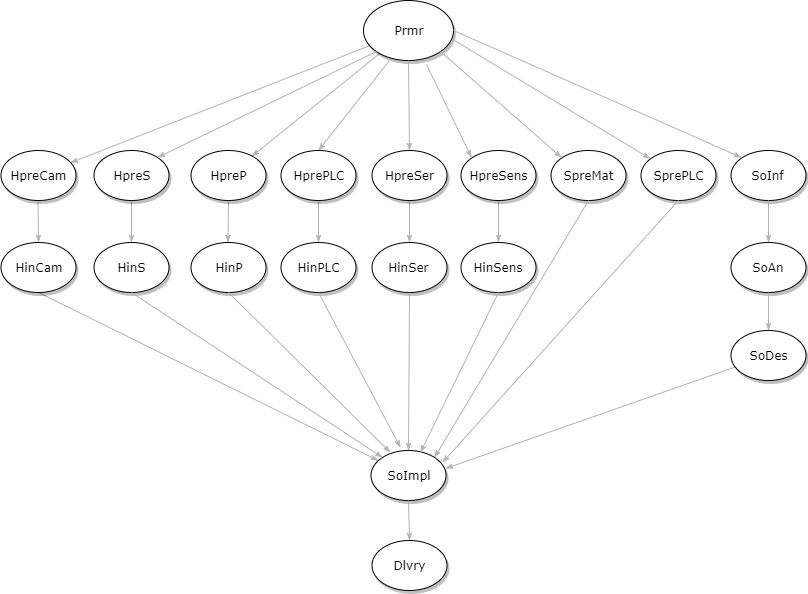
\includegraphics[width=\textwidth]{images/precedenceChart}
\end{figure}
\newpage
\section{Critical Path Method}
Once all tasks of a project have been defined, working times can be added. This allows determining how long the project takes, for example. There are tasks that can be started in parallel to others. However, this is not obvious at first glance. For this reason, this project uses the critical path method in conjunction with the GANTT diagram. Figure \ref{fig:criticalPath} shows the critical path in hatched structure. On the following page, see figure \ref{fig:pertChart}, a network plan on which the critical elements are provided with a thick red frame can be seen. 
\\
The critical path method is mainly used for projects that percentage of completion is calculable. Since this project has a fixed deadline, it makes sense to use the critical path method to pay particular attention to critical sections of the project.
\begin{landscape}
	% Header entfernt, damit das Bild mehr Platz hat
	\thispagestyle{plain}
	%\newgeometry{
	%  	left=3cm,
	%	right=3cm,
	%	top=2cm,
	%	bottom=4cm,
	%	bindingoffset=5mm
	%}
	\begin{figure}[h]
		\centering
		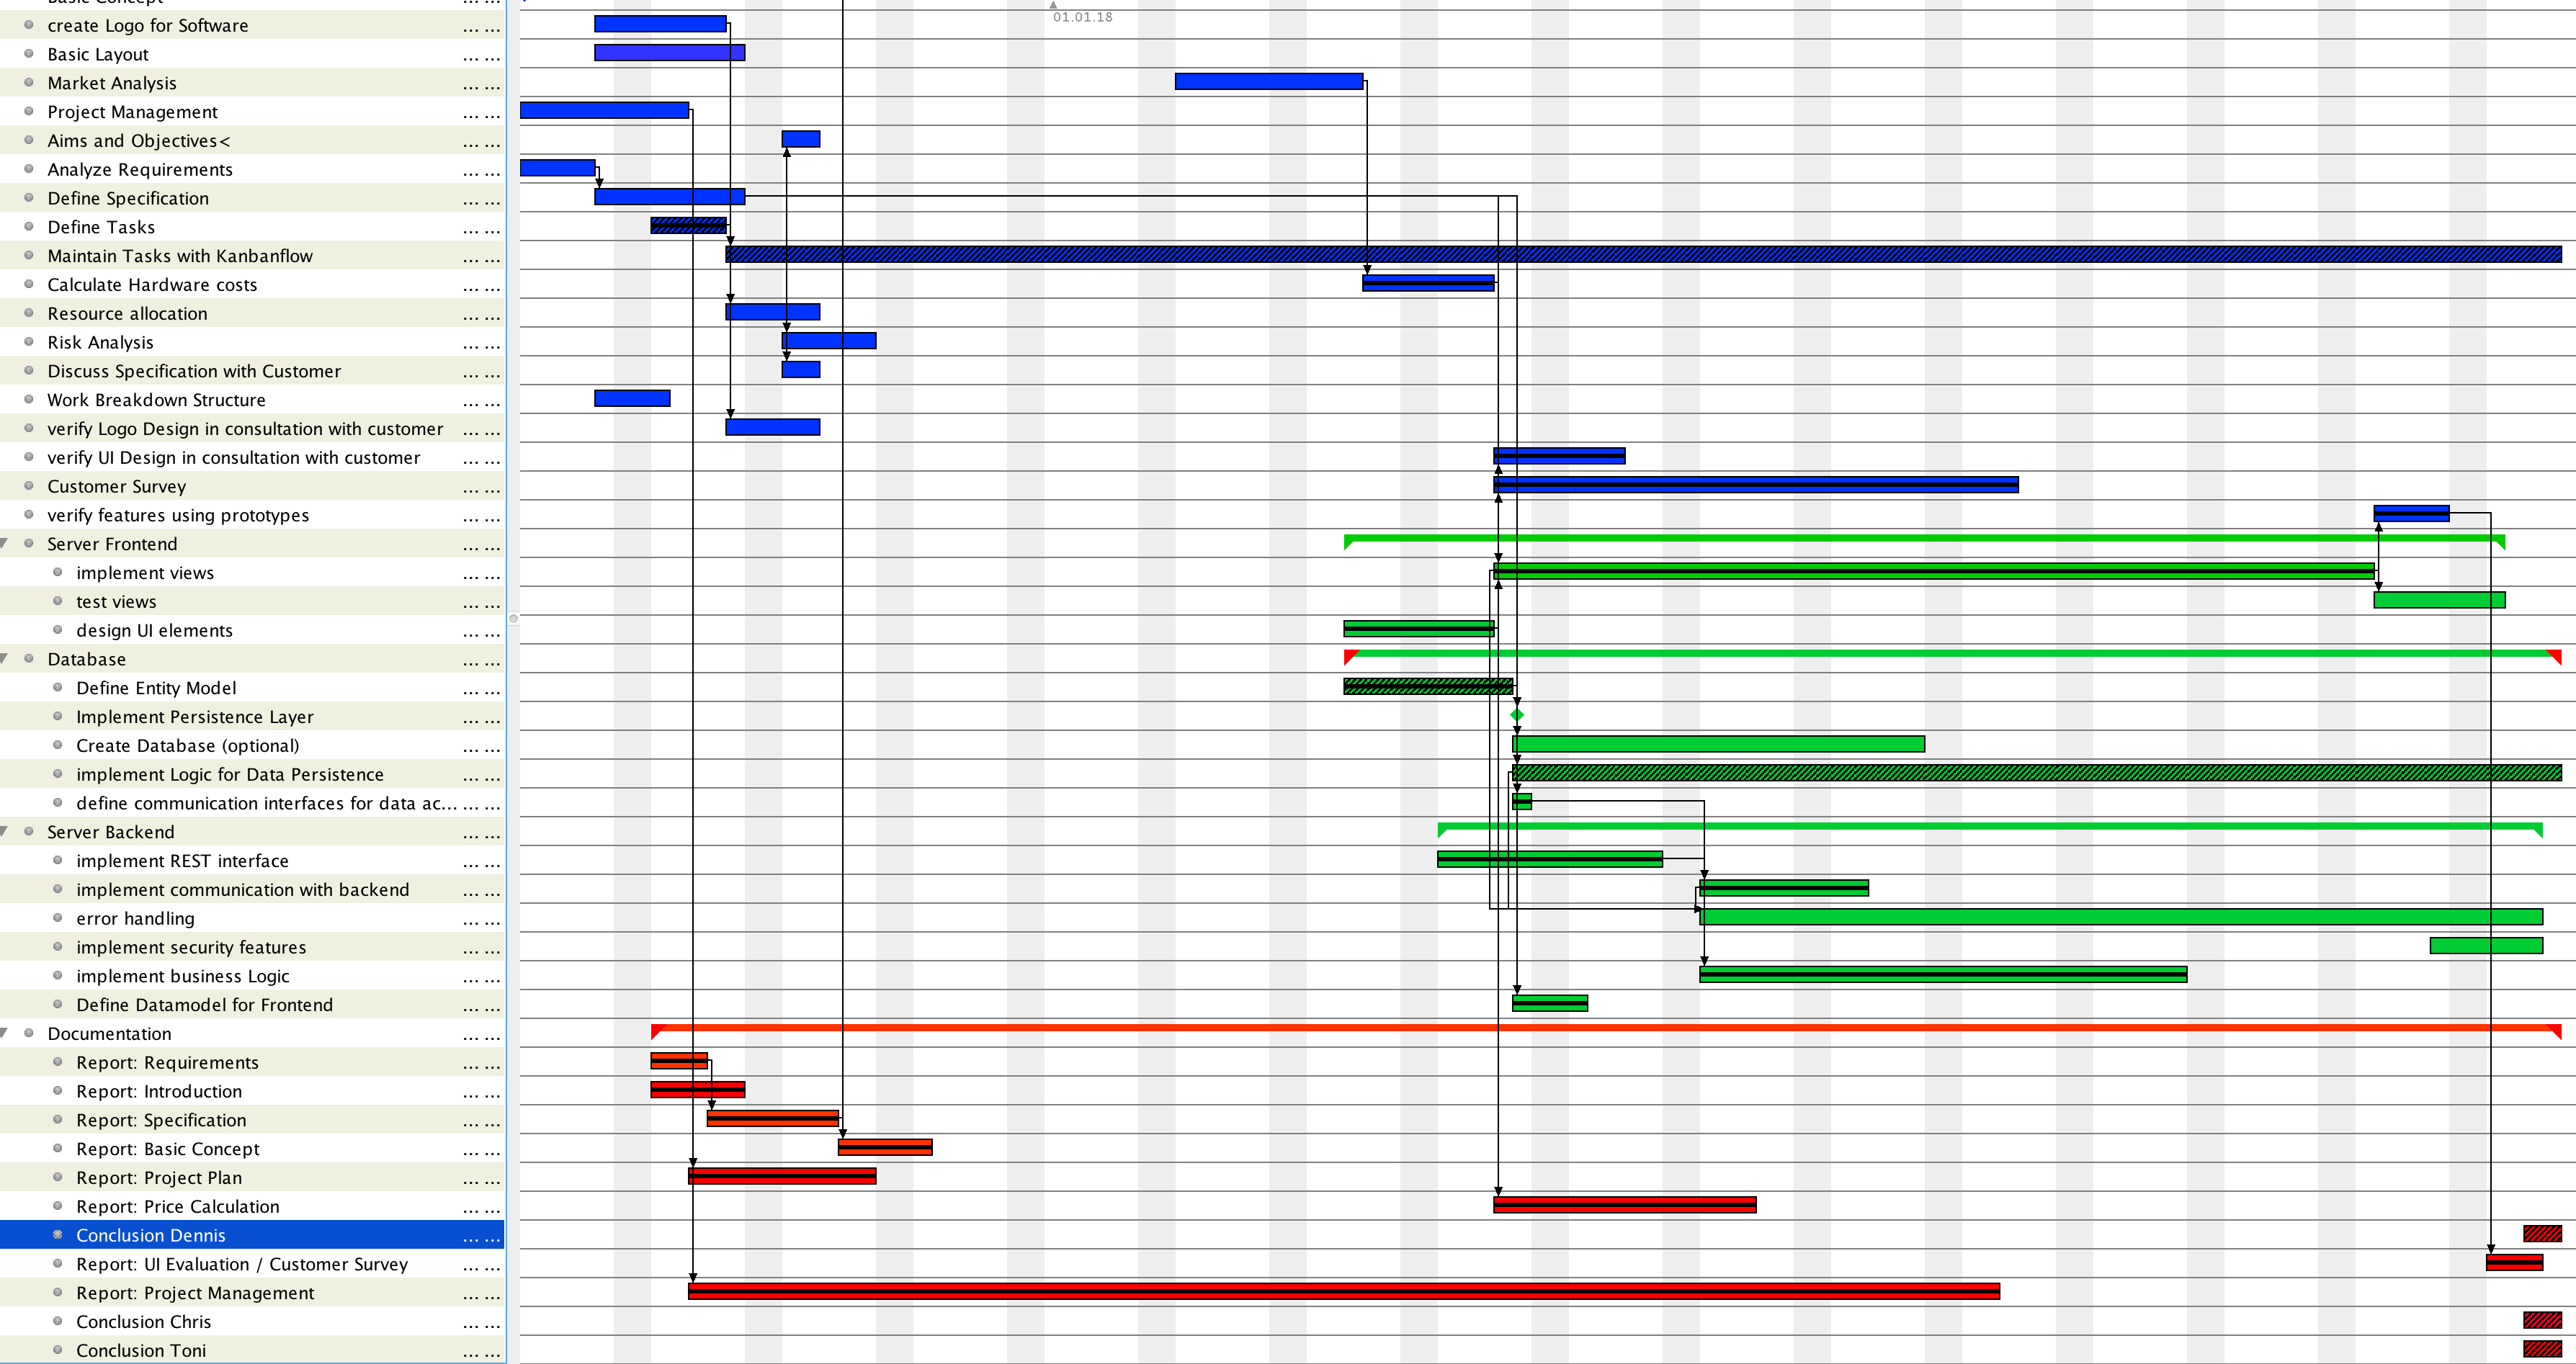
\includegraphics[width=1.4\textwidth]{images/criticalPath}
		\caption{Critical Path}
		\label{fig:criticalPath}
	\end{figure}
	\pagebreak
	% Header entfernt, damit das Bild mehr Platz hat
	\thispagestyle{plain}
	\begin{figure}[h]
		\centering
		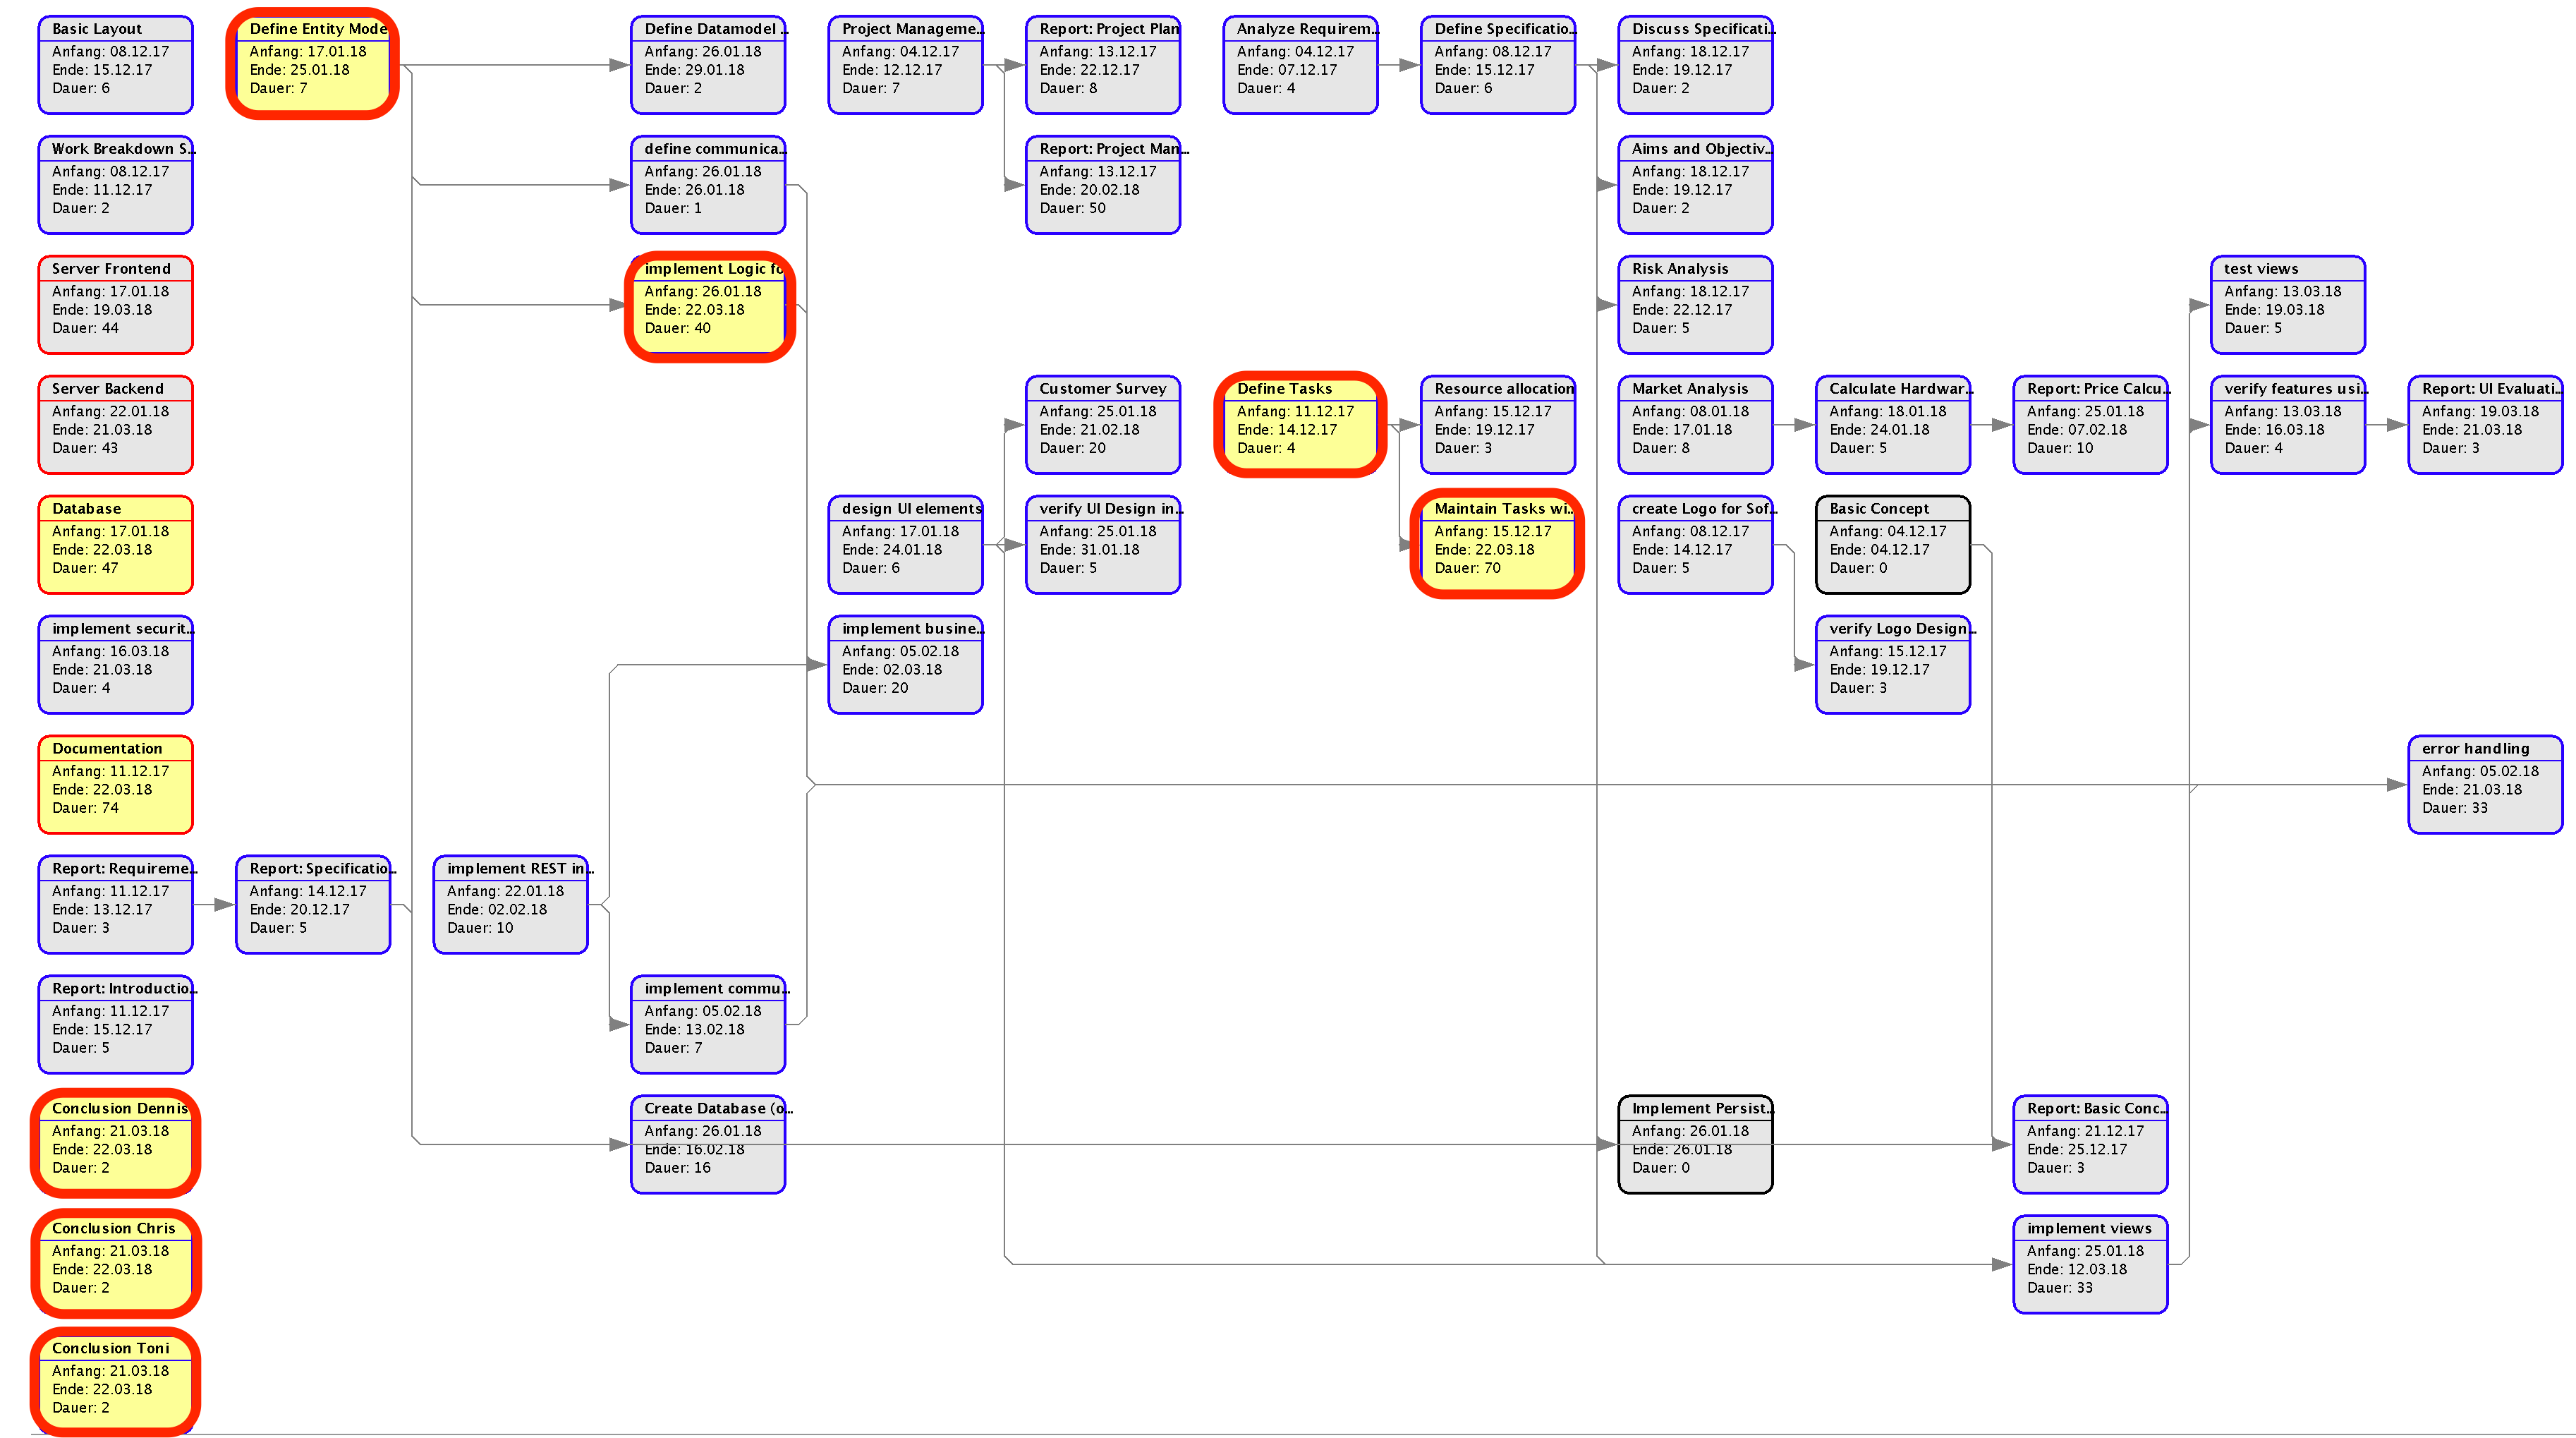
\includegraphics[width=1.4\textwidth]{images/pertChart}
		\caption{Network Plan with critical path}
		\label{fig:pertChart}
	\end{figure}
	%\restoregeometry
\end{landscape}

